\documentclass[]{article}
\usepackage[utf8]{inputenc}
\usepackage[T1]{fontenc}
\usepackage[switch]{lineno}
\usepackage{amsfonts,amsmath,amssymb}
\usepackage{graphicx,dcolumn,bm,xcolor,ulem}
\usepackage{hyperref,url}



\title{Ranking fútbol}
\author{}
\date{}

\begin{document}
	
\maketitle

\begin{abstract}
	We ...
\end{abstract}


\section{Introduction}

\section{Data}

\subsection{Recopilación de métricas}

En este trabajo utilizamos la base de datos de evento provista por L. Pappalardo et al en \cite{pappalardo2019public}. 
En ese articulo, los autores visualizan todos los partidos de la temporada 2017-2018 de las principales ligas de fútbol europeas: La Liga (España), Premier league (Inglaterra), Seria A (Italia), Bundesliga (Alemania), Ligue 1 (Francia). Por cada partido detectan, clasifican, y localizan en tiempo y espacio todos los eventos: goles, tiros al arco, pases, saques de esquina, faltas, etc. 
%
En el sistema de referencia que utilizan para ubicar los eventos en tiempo y espacio, $t$ expresa el tiempo transcurridos desde el inicio del partido, la coordenada $x$ expresa la distancia respecto del arco del equipo creador del evento, y la coordenada $y$ la distancia respecto a la banda lateral derecha. Las unidades de las coordenadas espaciales están dadas en porcentajes del campo juego, siendo por ejemplo $x=0$, $x=50$ y $x=100$ las posiciones de la linea de meta propia, la linea de centro del campo y la linea de meta del rival, respectivamente. 

En este marco, definimos intervalo de posesión de pelota (BPI) como al conjunto dado por una secuencia continua de eventos generados por un equipo. Note que cada BPI contiene información de un solo equipo.
Recopilamos todos los BPI de todos los equipos de cada liga, y sobre esos datos extrajimos algunas métricas que nos permiten detectar los recursos tácticos que están utilizando los equipos en esa ventana temporal del partido. 
Las métricas recopiladas para nuestro análisis están basadas en las propuestas por J. Fernandez-Navarro en \cite{fernandez2018influence}.
A continuación describimos en detalle a cada una de estas,

\begin{enumerate}
    \item {\it Direct play.} Cada vez que hay un pase o un tiro libre en un BPI, medimos la velocidad media en la dirección de ataque, dada por el cociente entre la distancia recorrida por la pelota en el eje $x$ y el tiempo transcurrido. De cada BPI tomamos el valor máximo. 
    Esto nos permite detectar que tan directo hacia la portería rival es el movimiento de la pelota en el equipo.

    \item {\it Counterattack.} Dado dos eventos consecutivos en un BPI, si el primero se observa en $x_1<40$ y el segundo en $x_2>60$ a una diferencia temporal $\Delta t$, se informa la velocidad como $v=\frac{x_2-x_1}{\Delta t}$. En otro caso se informa $0$.
    Esto es una medida de que tan rápido un equipo pasa de una posición defensiva en su campo a una ofensiva en campo rival.

    \item {\it Maintenance.} Dado un BPI, se calcula el promedio de las posiciones en el eje $x$, donde se generaron todos los eventos. Si se cumple $\bar{x}<40$, es decir si los eventos se desarrollaron mayoritariamente en la zona defensiva del equipo,
    se informa el tiempo total de la posesión. En otro caso se informa $0$. Esto nos permite detectar que tanto un equipo decide mantener y construir su juego desde su propio campo.

    \item {\it Build up.} Si en un BPI se verifica que $\bar{x}>60$, es decir la posesión se desarrolla mayoritariamente en campo rival, se informa el tiempo total de la posesión. En otro caso se informa $0$. Esta métrica informa el tiempo de posesión en situaciones donde el equipo invade fuertemente el campo rival.   

    \item {\it Midfield play.} Si en un BPI se observa que $\bar{x}\leq60$ y $\bar{x}\geq40$, es decir la posesión de desarrolla mayoritariamente por el centro del campo de juego, se informa el tiempo total de la posesión, en otro caso se informa $0$.La idea de esta variable es medir el tiempo que el equipo pasa en el sector medio del campo de juego.

    \item {\it Flow rate.} En cada BPI donde $\bar{x}\geq50$ se toma la diferencia temporal entre todos los eventos, y se calcula el valor medio, $\bar{dt}$. Luego se define la métrica como $1/\bar{dt}$. De esta manera se tiene una medida de que tan rápido el equipo mueve la pelota en el campo rival.

    \item {\it Crossing.} Si en un BPI se observa un evento centro, se informa $1$, en otro caso se informa $0$. Esta métrica sirve para contabilizar los intentos de llegada por vía aérea.

    \item {\it Pressure point.} De cada BPI se toma el primer evento, y se extrae la posición en la variable $x$, es decir donde el equipo comienza su posición. Esto nos permite medir si el equipo esta recuperando la pelota en su campo, en la zona media o en el campo rival.
 
    \item {\it Pressure loss.} Si un BPI comienza en un evento donde $x>40$, se informa el tiempo total de la posesión del adversario del BPI inmediatamente anterior. Este métrica es útil para observar si el equipo esta relajando o aumentando el nivel de presión que ejerce sobre el juego del rival en las zonas medias y altas del campo de juego.

    \item {\it Shots.} Si en un BPI se registra un evento ``Shot", se informa 1, en otro caso se informa $0$. Esta métrica permite contabilizar los tiros al arco de cada equipo.
    
\end{enumerate}

Para nuestro análisis,se descartaron todas los BPI con menos de 3 eventos y con tiempo total menor a 2 segundos. La idea de esto es descartar pequeñas recuperaciones pasajeras y quedarnos con posesiones consolidadas.
Del proceso de recopilación se obtuvieron $215681$ BPI.
%
%Luego de calcular los valores de las métricas en cada uno de estos, estudiamos la distribución de los datos. Observamos que las métricas parecen seguir una distribución tipo log-normal, por lo tanto decidimos transformar los datos como $x \rightarrow log(1+x)$ para trabajar con distribuciones aproximadamente normales. 
%
Luego, agrupamos la información por partido y por equipo, y sumamos los valores obtenidos en cada métrica. De esta manera por ejemplo el feature {\it Shots} cuantifica la cantidad de tiros al arco ejecutados por el equipo en ese partido.
Asimismo el feature {\it Build-up} cuantifica la cantidad de tiempo neto en la cual un equipo sostuvo una posición de ataque frente al rival en ese partido.
%
Note que en la temporada 2017/2018, en las ligas Española, Inglesa, Francesa e Italiana los equipos jugaron 38 partidos. Por lo tanto, al tomar los datos de los primeros 4 equipos cada liga aporta un total de $38\times4=152$ muestras al archivo de datos. Asimismo, en la liga alemana, al ver menos equipos, se jugaron 34 partidos, por lo tanto esta liga aporta 136 muestras. 
%
En consecuencia, DS es una matriz con 744 filas y 10 columnas. 
Por ultimo, en un dataset aparte recopilamos meta data asociada a cada muestra, útil luego para realizar el análisis: a que equipo pertenece esa muestra, cual es la liga de pertenencia, y el resultado final en la tabla de posiciones. 

\subsection{Representación en redes complejas}

En lo que sigue, presentamos nuestra propuesta para representar las métricas de rendimiento en términos de redes complejas.
Definimos $M(i, j, g)$ como la métrica de rendimiento correspondiente al equipo $i$ cuando enfrenta al equipo $j$ en el partido $g$. Por ejemplo, puede representar la cantidad de tiros al arco realizados por el FC Barcelona al jugar contra el Real Madrid en el primer encuentro del torneo español {\it La Liga}.
%
En nuestro conjunto de datos, todos los equipos participaron en un formato de liga todos contra todos, enfrentándose dos veces: un partido de ida ($g_1$) y otro de vuelta ($g_2$). Utilizando la información de ambos encuentros, definimos una métrica agregada que resume el desempeño observado entre esos dos equipos a lo largo del torneo:

$$
M(i,j) = \sum_{g_1, g_2} M(i,j,g).
$$
%
En el ejemplo anterior, $M(i,j)$ representa la cantidad total de tiros al arco realizados por el FC Barcelona contra el Real Madrid en ambos partidos del torneo.
%
Calculando $M(i,j)$ para cada par de equipos en una liga $L$, es posible representar estas relaciones de desempeño mediante un grafo dirigido y ponderado $G(L,M)$, cuyos pesos se definen como

$$
f_{ij} = M(j,i) - M(i,j).
$$
%
Nótese que, en esta representación, $f_{ij} < 0$ indica que el equipo $i$ superó al equipo $j$ en la métrica considerada.
%
En este marco, construimos diez grafos por liga, cada uno asociado a una métrica de rendimiento distinta.












\section{Resultados}

\subsection{Caracterización estructural de las redes}


\subsection{Calculo de rating mediante descomposición de Hodge }


\subsection{Comparación con el rating real en cada liga}


\section{Conclusion}



\begin{figure}[t!]
\centering
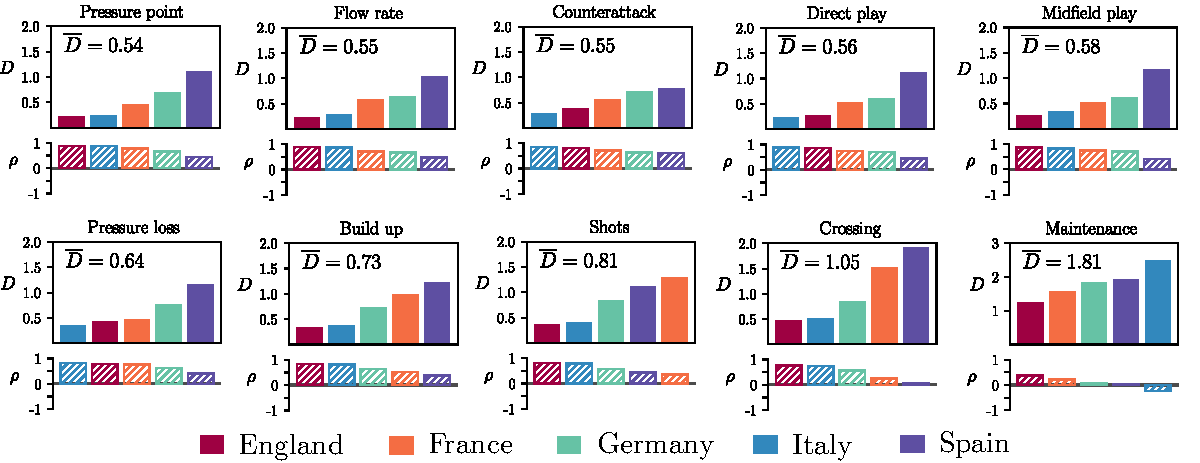
\includegraphics[width=1.\textwidth]{metricas.pdf}
\caption{ORIGINAL}
\label{}
\end{figure}


\begin{figure}[t!]
\centering
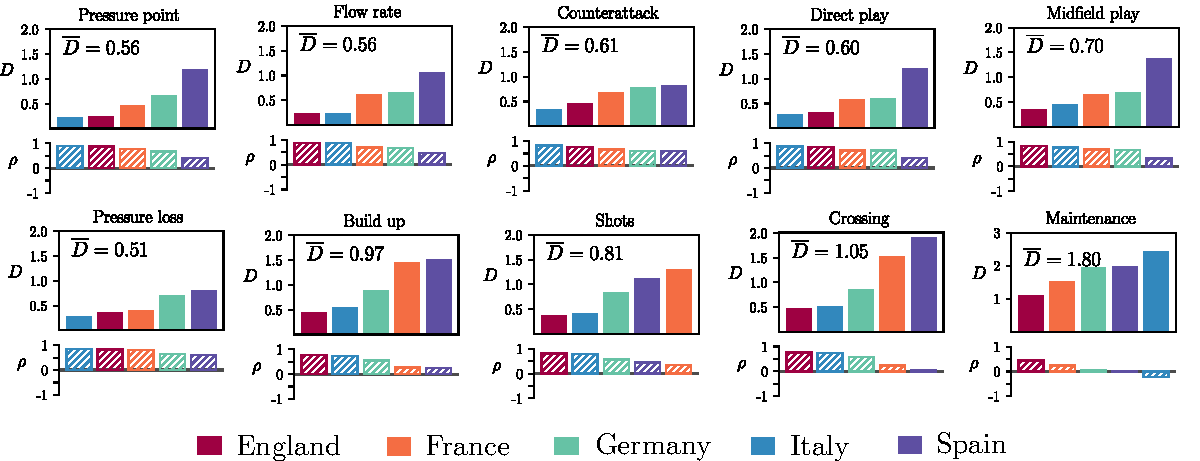
\includegraphics[width=1.\textwidth]{fig_all_2.pdf}
\caption{CAMBIO NORMALIZACIÓN (ALL2) }
\label{}
\end{figure}


\begin{figure}[t!]
\centering
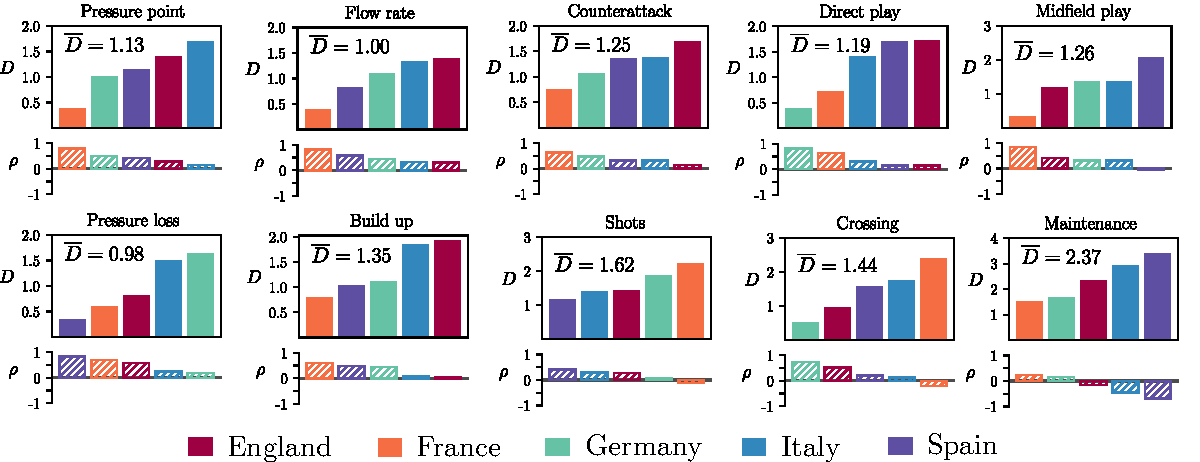
\includegraphics[width=1.\textwidth]{ffig_first6.pdf}
\caption{FIRST 6}
\label{}
\end{figure}


\begin{figure}[t!]
\centering
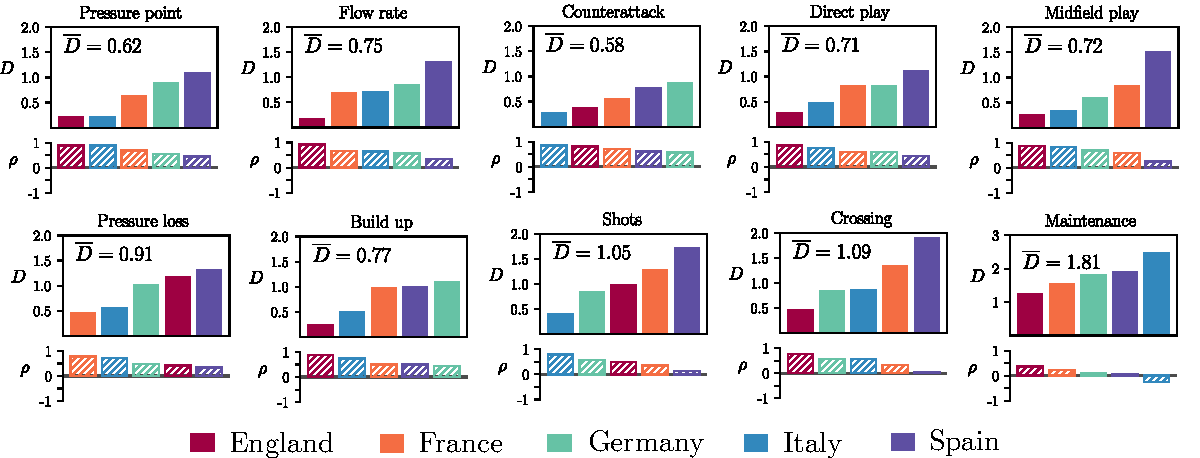
\includegraphics[width=1.\textwidth]{fig_mst.pdf}
\caption{MST}
\label{}
\end{figure}





\bibliographystyle{unsrt}
\bibliography{biblio}


%%%%%%%%%%%%%%%%%%%%%%%%%%%%%%%%%%%%%%%%%%%%%%%%%%%

	
\end{document}